\documentclass[a4paper,10pt,twoside]{article}
%%%%%%%%%%% Packages %%%%%%%%%%
\usepackage[margin=1in]{geometry}
\usepackage{amsmath, amssymb,mathtools}
\usepackage{fancyhdr}
\usepackage{sectsty}
\usepackage{enumitem}
\usepackage{float}
\usepackage{braket}
\usepackage{bbm}
\usepackage{tikz,calc}
\usepackage{amsthm}


%%%%%%%%%%% Macros %%%%%%%%%%
\def \note#1 {\vspace{-1em}\paragraph{\bfseries #1}}
\def \dd {{\rm d}}
\def \id {{\mathbbm{1}}}
\def \order {\mathcal{O}}
\def\bquad{\mkern-18mu}
\DeclareMathOperator{\trace}{tr}
\DeclareMathOperator{\spanset}{span}

%%%%%%%%%%% Tikz Definitions %%%%%%%%%%
\usetikzlibrary{shapes, arrows,positioning,fit}
\tikzstyle{plain} = [draw,thick,circle,inner sep=0,minimum size=0.5cm,font=\footnotesize]
\tikzstyle{mps} = [draw,thick,rectangle,rounded corners=.1cm,inner sep=0,minimum size=0.5cm]
\tikzstyle{mpo} = [draw,thick,circle,inner sep=0,minimum size=0.5cm]
\tikzstyle{index} = [-,thick,font=\footnotesize]
\tikzstyle{virtual} = [-,thick,dotted,font=\footnotesize]

\def \tu {0.25cm}

%%%%%%%%%%% Formatting %%%%%%%%%%
\pagestyle{fancy}
\renewcommand{\footrulewidth}{0.5pt}

\fancyhf{}
\lhead{04/05/2017}
\chead{Quantum Information Methods in Many-Body Physics}
\rhead{PH2269}
\lfoot{Giacomo Giudice~~~~giacomo.giudice@mpq.mpg.de}
\rfoot{Page \thepage}

\allsectionsfont{\normalfont\sffamily}

\newtheoremstyle{modern}{3pt}{3pt}{\itshape}{}{\sffamily\bfseries}{}{.5em}{}
\theoremstyle{modern}
\newtheorem{lemma}{Lemma}[section]
\newtheorem{theorem}[lemma]{Theorem}

%%%%%%%%%%% Here Begins Document %%%%%%%%%%
\begin{document}
\title{\vspace{-1cm}\sffamily Solutions to Homework 3\vspace{-1cm}}
\author{}
\date{}
\maketitle
\thispagestyle{fancy}

\begin{section}{}
Using the definition of an MPS,
\[
  \braket{{\Psi}|{\Psi}} = \sum_{\{i_n\}}\overline{\trace(A^{i_1}\dots A^{i_N})}\trace(A^{i_1}\dots A^{i_N})
  = \trace \left(\sum_{i_1} \bar{A}^{i_1} \otimes A^{i_1}\right) \dots \left(\sum_{i_N} \bar{A}^{i_N} \otimes A^{i_N}\right)
  = \trace{\mathbb{E}^N}.
\]
Using the fact that $r$ and $\ell$ are the fixed points of $\varepsilon$ and $\varepsilon^*$ respectively,
\[
  \sum_i \tilde{A}^{i\dag} \tilde{A}^i = \sum_i \ell^{-1/2} \underbrace{{A^{i}}^\dag \ell^{1/2} \ell^{1/2} A^i }_{=\ell} \ell^{-1/2} = \id, \quad \sum_i \tilde{A}^i \tilde{A}^{i\dag} = \sum_i r^{-1/2} \underbrace{A^i r^{1/2} r^{1/2} {A^i}^\dag }_{=r} r^{-1/2} = \id .
\]
Graphically, the left-canonical form corresponds to
\[
  {
  \tikz[baseline=-2*\tu,node distance=\tu]{
      \node[mps] (mconj) {$\bar{A}$};
      \node[mps,below=of mconj] (m) {$A$};
      \draw[index] (m.west) to[in=180,out=180] (mconj.west);
      \draw[index] (m.north) -- (mconj.south);
      \draw[index] (mconj.east) -- +(\tu,0);
      \draw[index] (m.east) -- +(\tu,0);
      \useasboundingbox (0,-\tu) rectangle (1*\tu,\tu);
    }
  }
  = 
  {
  \tikz[baseline=-2*\tu,node distance=\tu]{
      \node[] (gconj) {};
      \node[below=2*\tu of gconj] (g) {};
      \draw[index] (g.west) to[in=180,out=180] (gconj.west);
    }
  }
  \qquad
  {
  \tikz[baseline=-2*\tu,node distance=\tu]{
      \node[mps] (mconj) {$\bar{A}$};
      \node[mps,below=of mconj] (m) {$A$};
      \node[fit=(mconj)(m)] (f) {};
      \node[plain,right=0 of f] (rho) {$\rho$};
      \draw[index] (rho.north) to[in=0,out=145] (mconj.east);
      \draw[index] (rho.south) to[in=0,out=-145] (m.east);
      \draw[index] (m.north) -- (mconj.south);
      \draw[index] (mconj.west) -- +(-\tu,0);
      \draw[index] (m.west) -- +(-\tu,0);
    }
  }
  = 
  {
  \tikz[baseline=-0.5*\tu,node distance=\tu]{
      \node[plain] (rho) {$\rho$};
      \draw[index] (rho.north) to[in=0,out=90] +(-0.5*\tu,0.5*\tu);
      \draw[index] (rho.south) to[in=0,out=-90] +(-0.5*\tu,-0.5*\tu);
    }
  }
\]
\begin{theorem}[Fundamental theorem of MPS]
\end{theorem}
\begin{proof}
In the large $N$ limit, the overlap is $|\braket{{\Psi}_B|{\Psi}_A}| \to |\lambda|^N$. 
Clearly, $|\lambda| \leq 1$, and there are two possible scenarios in the termodynamic limit:
\begin{itemize}
  \item $|\braket{{\Psi}_B|{\Psi}_A}| \to 0$, if the two states are different ($\lambda < 1$),
  \item $|\braket{{\Psi}_B|{\Psi}_A}| = 1$, if the two states are the same ($\lambda = 1$).
\end{itemize}
Hence, we are interested in the case where $\lambda = 1$.
Using the fact that the fixed point $\rho$ is strictly positive, 
\begin{align*}
   \left|\lambda \trace(X \rho X^\dag)\right|^2 &= \left| \trace(X A^i \sqrt{\rho}\sqrt{\rho} X^\dag {B^i}^\dag) \right|^2 \\
   &\leq \left(\sum_i \trace(X A^i \rho {A^i}^\dag X^\dag)\right) \! \left(\sum_i \trace(B^i X \rho X^\dag {B^i}^\dag)\right) = \left| \trace(X \rho X^\dag)\right|^2
\end{align*}
Since $\lambda = 1$, the Cauchy--Schwarz inequality is satisfied with an equal sign, that means that $u \propto v$, i.e. $X A^i \sqrt{\rho} = \alpha B^i X \sqrt{\rho}$.
and show that $\alpha$ must be unity since 
\[
  X = \sum_i {B^i}^\dag B^i X = \alpha \sum {B^i}^\dag X A^i = \alpha \lambda X.
\]
We can also absorb it into $X$. Since $\rho$ is full rank, it can be inverted,
\[
  XA^i = B^i X.
\] 
\end{proof}
\note{Note} A diagrammatic proof has been shown during the exercise session.
\end{section}

\begin{section}{}
Calculating the sum explicitly yields $\sum_\sigma {A^\sigma}^\dag A^\sigma = \frac{3}{4}\id$. 
Therefore we rescale all $A^\sigma$ by $2/\sqrt{3}$,
\[
  A^+=\frac{2}{\sqrt{3}}
  \begin{pmatrix}
    0 & 1\\
    0 & 0
  \end{pmatrix}, \quad
  A^0=\frac{1}{\sqrt{3}}
  \begin{pmatrix}
    -1 & 0\\
    0 & 1
  \end{pmatrix}, \quad
  A^-=\frac{2}{\sqrt{3}}
  \begin{pmatrix}
    0 & 0\\
    -1 & 0
  \end{pmatrix}.
\]
Calculating the transfer matrix yields
\[
  \mathbb{E} = \frac{1}{4}
  \begin{pmatrix}
    1 & 0 & 0 & 2\\
    0 & -1 & 0 & 0\\
    0 & 0 & -1 & 0\\
    2 & 0 & 0 & 1\\
  \end{pmatrix}.
\]
The eigenvalues are $1$, $-1/3$, $-1/3$, $-1/3$.
Therefore, $\braket{\Psi|\Psi} = 1 + 3(1/3)^L \to 1$ as $L \to \infty$.
\end{section}

\begin{section}{}
After blocking $L$ sites, we still have only two linear independent vectors, namely $\ket{0,\dots,0} = A^0 \dots A^0$ and $\ket{1,\dots,1} = A^1 \dots A^1$. 
Therefore, we will never be able to span a space of $2 \times 2$ with two vectors, hence this state will never be injective by blocking, we say its \emph{injectivity length} is infinite.
We also notice that GHZ state is scale-invariant.
The transfer matrix is 
\[
  \mathbb{E} = 
  \begin{pmatrix}
    1 & 0 & 0 & 0\\
    0 & 0 & 0 & 0\\
    0 & 0 & 0 & 0\\
    0 & 0 & 0 & 1
  \end{pmatrix},
  \quad
  \ket{\rho_\uparrow} = 
  \begin{pmatrix}
    1\\
    0\\
    0\\
    0\\
  \end{pmatrix},
  \quad
  \ket{\rho_\downarrow} = 
  \begin{pmatrix}
    0\\
    0\\
    0\\
    1\\
  \end{pmatrix},
\]
it has two degenerate dominant eigenvalues $1$, with associated eigenvectors $\ket{\rho_\uparrow}$ and $\ket{\rho_\downarrow}$.
Notice that $\mathbb{E}^N =  \mathbb{E} = \ket{\rho_\uparrow}\bra{\rho_\uparrow} + \ket{\rho_\downarrow}\bra{\rho_\downarrow}$.
Therefore,
\begin{align*}
  \braket{{\rm GHZ} | {\rm GHZ}} &= \trace \mathbb{E}^N =  \sum_{\mathclap{\mu = \uparrow,\downarrow}}  \braket{\rho_\mu | \rho_\mu} = 2 \\
  \braket{O_n} &= \frac{1}{2}\trace({\mathbb{E}_O \mathbb{E}^N}) = \frac{1}{2} \sum_{\mathclap{\mu = \uparrow,\downarrow}}  \braket{\rho_\mu | \mathbb{E}_O | \rho_\mu}, \\
  \braket{O_n O_{L+n}} &= \frac{1}{2}\trace({\mathbb{E}_O \mathbb{E}^{L-1} \mathbb{E}_O \mathbb{E}^N}) =  \frac{1}{2}\sum_{\mathclap{\mu,\nu = \uparrow,\downarrow}} \braket{\rho_\mu | \mathbb{E}_O | \rho_\nu} \braket{\rho_\nu | \mathbb{E}_O | \rho_\mu}  \\
  C_L &=  \frac{1}{4} \sum_{\mathclap{\mu,\nu = \uparrow,\downarrow}} 2 \braket{\rho_\mu | \mathbb{E}_O | \rho_\nu}\braket{\rho_\nu | \mathbb{E}_O | \rho_\mu} - \braket{\rho_\mu | \mathbb{E}_O | \rho_\mu}\braket{\rho_\nu | \mathbb{E}_O | \rho_\nu}\\
  &=  \frac{1}{4} \bigg( |(\mathbb{E}_O)_{\uparrow\uparrow}|^2  + 4 (\mathbb{E}_O)_{\uparrow\downarrow}(\mathbb{E}_O)_{\downarrow\uparrow} - 2 (\mathbb{E}_O)_{\uparrow\uparrow}(\mathbb{E}_O)_{\downarrow\downarrow}  + |(\mathbb{E}_O)_{\downarrow\downarrow}|^2   \bigg), 
  \quad 
  (\mathbb{E}_O)_{\mu\nu} = \braket{\rho_\mu | \mathbb{E}_O | \rho_\nu}.
\end{align*}
Notice how the correlation is independent of $L$. The GHZ has \emph{infinite-range correlation}, and, somewhat surprisingly, we can describe that with a non-normal MPS.
\end{section}

\begin{section}{}
We simply repeat the results in the original paper\footnote{N. Schuch, J.I. Cirac, D. Per{\'e}z-Garc{\'i}a, Annals of Physics (2010), arXiv:1001.3807. \\ All diagrams of this exercise come from this paper.}.
If some steps are not clear, you should take a look at it.
Graphically, the inverse acts as
\[
  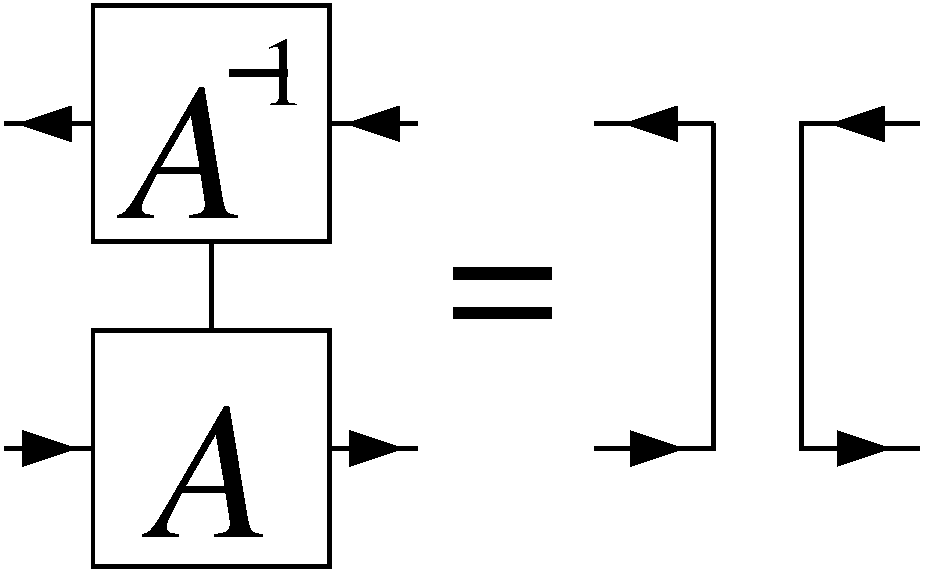
\includegraphics[height=3em]{diagrams/linv}
\]
The injectivity is preserved by concatenating tensors, since
\[
  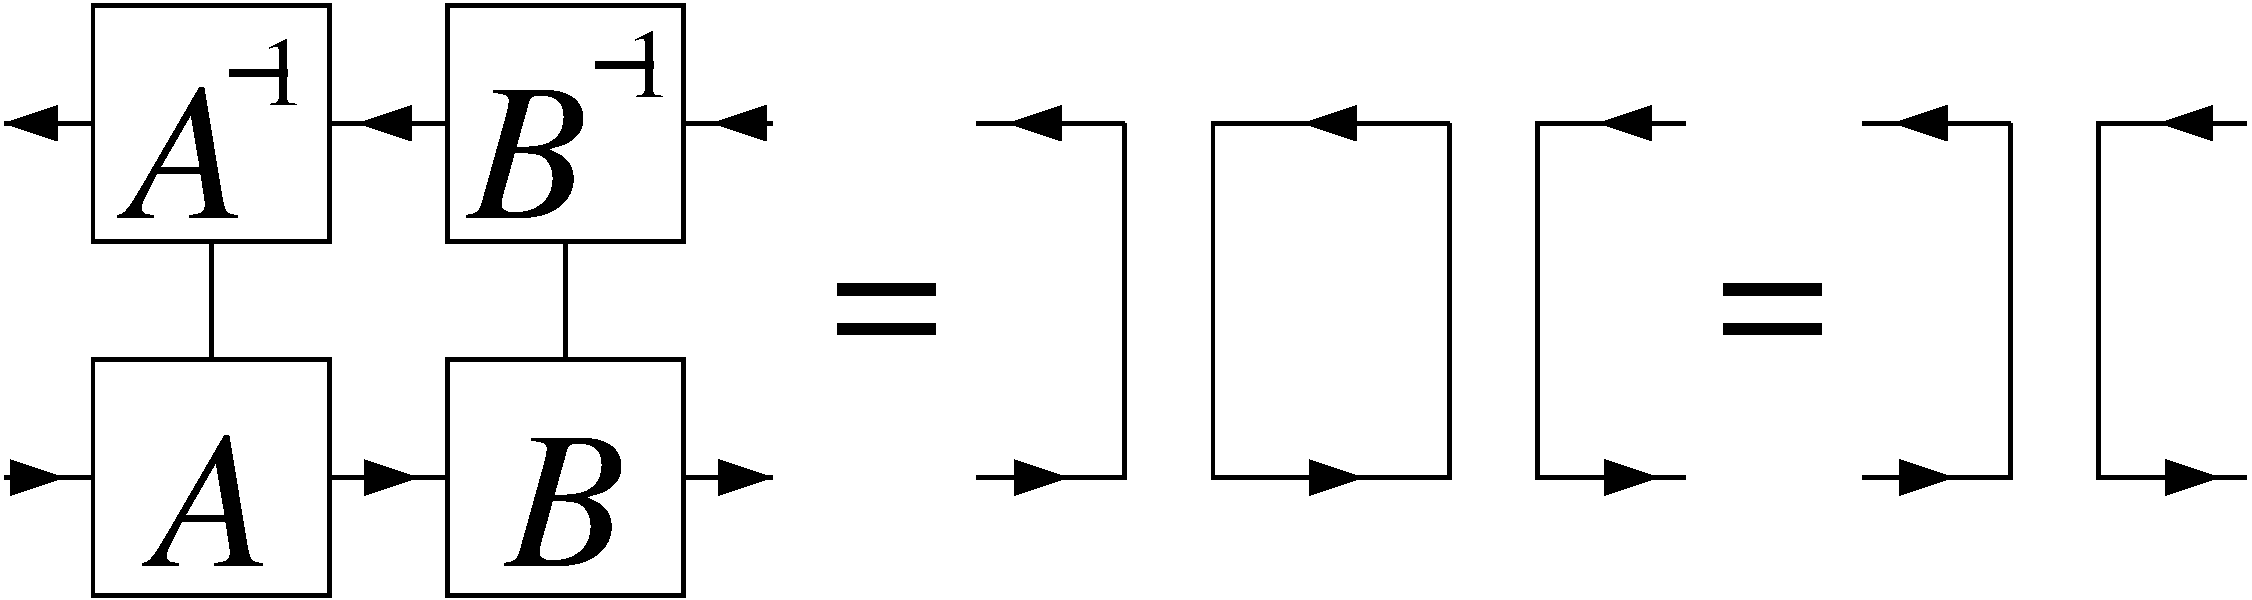
\includegraphics[height=3em]{diagrams/grow-inj}
\]
where we omit the scalar, corresponding to the contraction of the loop $\trace\id = D$. 

The $k$-site state is 
\[
  \Ket{\Psi^{[k]}_{i_{k+1},\dots,i_L}} = \sum_{\mathclap{i_1,\dots,i_k}}\trace(A^{i_1}\dots A^{i_k} X^{i_{k+1},\dots,i_L}) \ket{i_1,\dots,i_k}, \quad
  X^{i_{k+1},\dots,i_L} = A^{i_{k+1}} \dots A^{i_L}.
\]
The $k$-site density matrix $\rho_k$ is then
\[
 \rho_k = \sum_{i_{k+1},\dots,i_L}  \Ket{\Psi^{[k]}_{i_{k+1},\dots,i_L}} \Bra{\Psi^{[k]}_{i_{k+1},\dots,i_L}}
\]
We can think of this operator as a linear combination of outer products of elements in $\mathcal{S}_k$, hence a map $\rho_k: \mathcal{S}_k \mapsto \mathcal{S}_k$.
Moreover, it can be shown that the injectivity of $A$ implies that $ X^{i_{k+1},\dots,i_L}$ spans the whole space $\mathbf{L}(\mathbb{C}^{D \times D})$.

\begin{theorem}[Intersection property]
\label{tm:intersection}
\end{theorem}
\begin{proof}
To prove ${\rm rhs} \subseteq {\rm lhs}$ we choose
\[
  \raisebox{-1.3em}{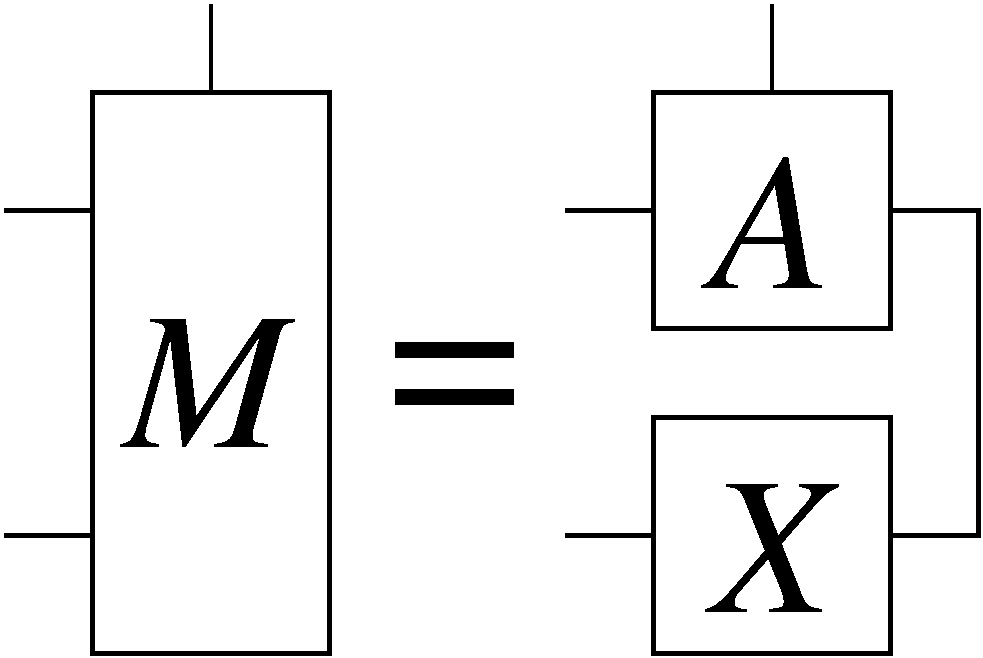
\includegraphics[height=3.2em]{diagrams/M-eq-BX}}\mbox{\quad and \quad}
  \raisebox{-1.3em}{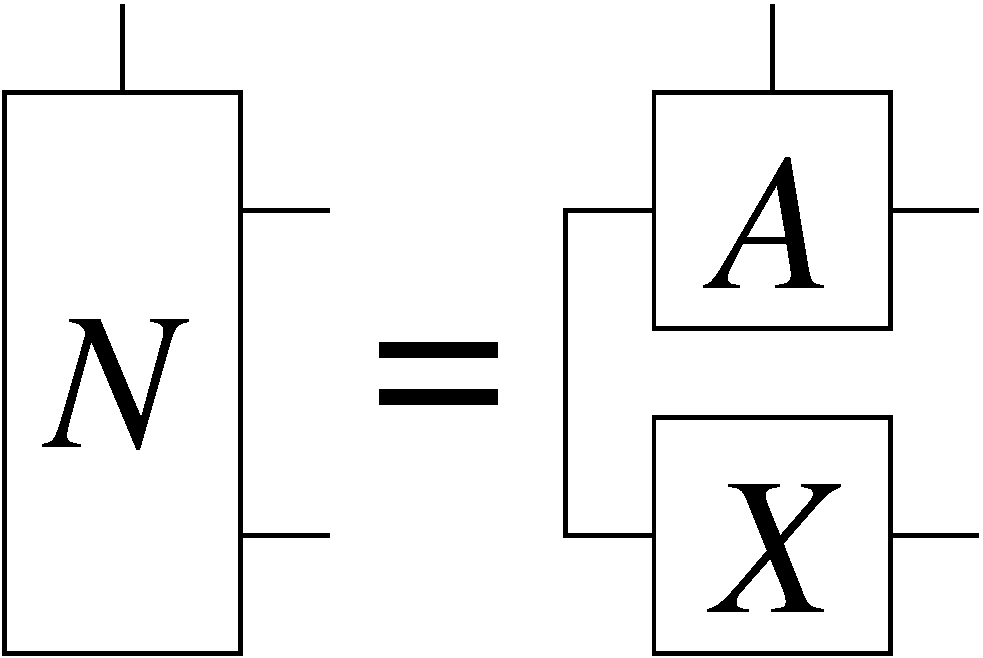
\includegraphics[height=3.2em]{diagrams/N-eq-BX}}\ .
\]
In the opposite direction, we obtain a relationship between $M$ and $N$ 
\[
  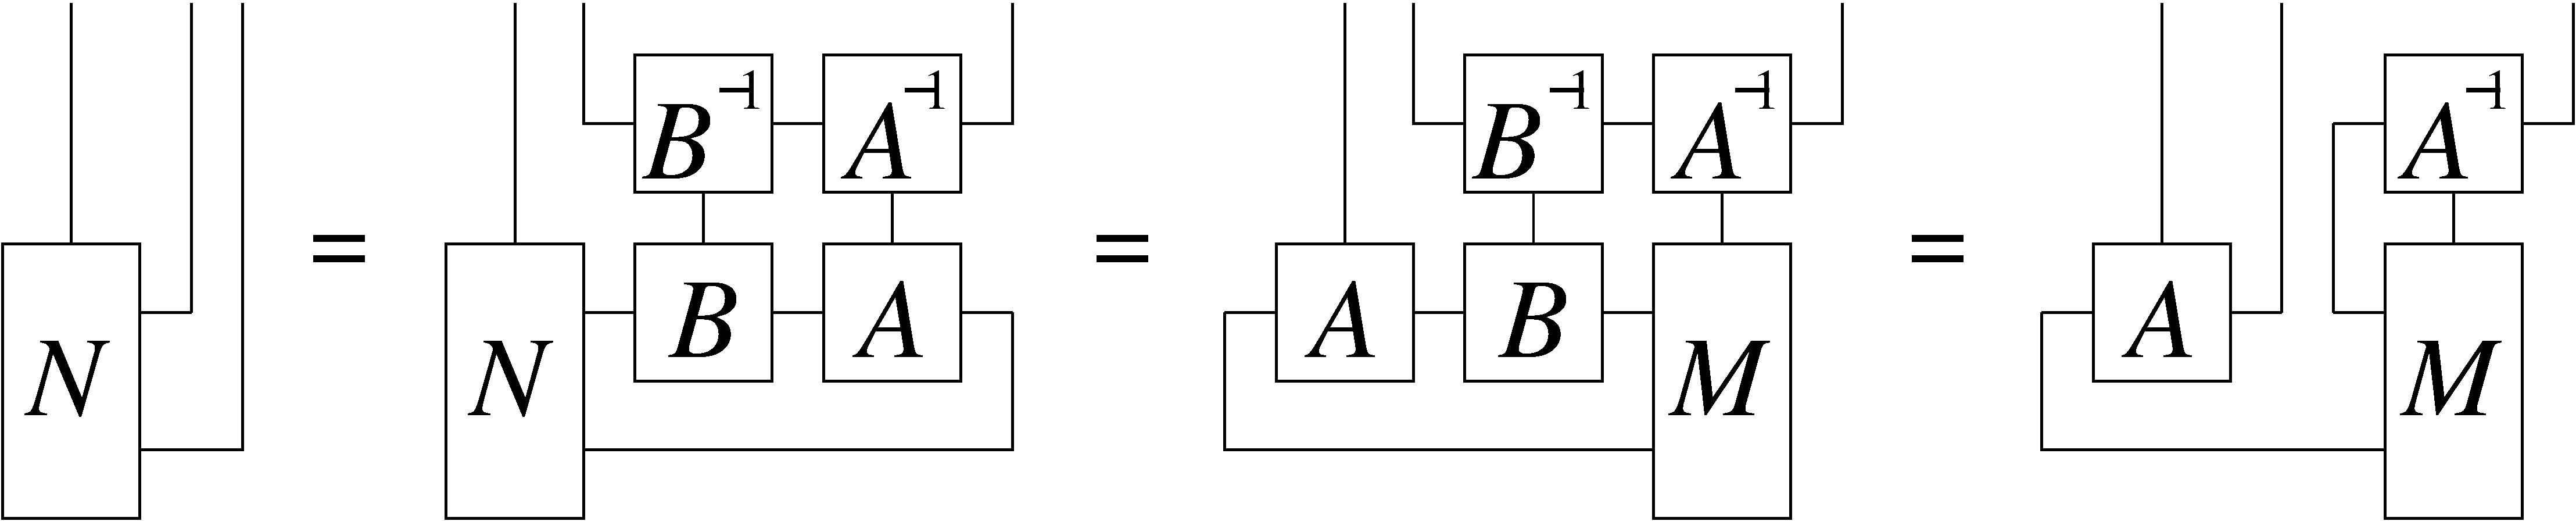
\includegraphics[height=4.5em]{diagrams/prove-N-eq-BX}\ ,
\]
which we plug back into $\ket{\psi}$ to obtain $\ket{\psi} \in {\rm rhs}$.
Hence ${\rm lhs} \subseteq {\rm rhs} \subseteq {\rm lhs} \Leftrightarrow {\rm lhs} = {\rm rhs}$.
\end{proof}
\begin{theorem}[Closure property]
\label{thm:closure}
\end{theorem}
\begin{proof}
The fact that ${\rm rhs} \subseteq {\rm lhs}$ is verified immediately by taking $M=N=\id$.
Conversely,
\[
  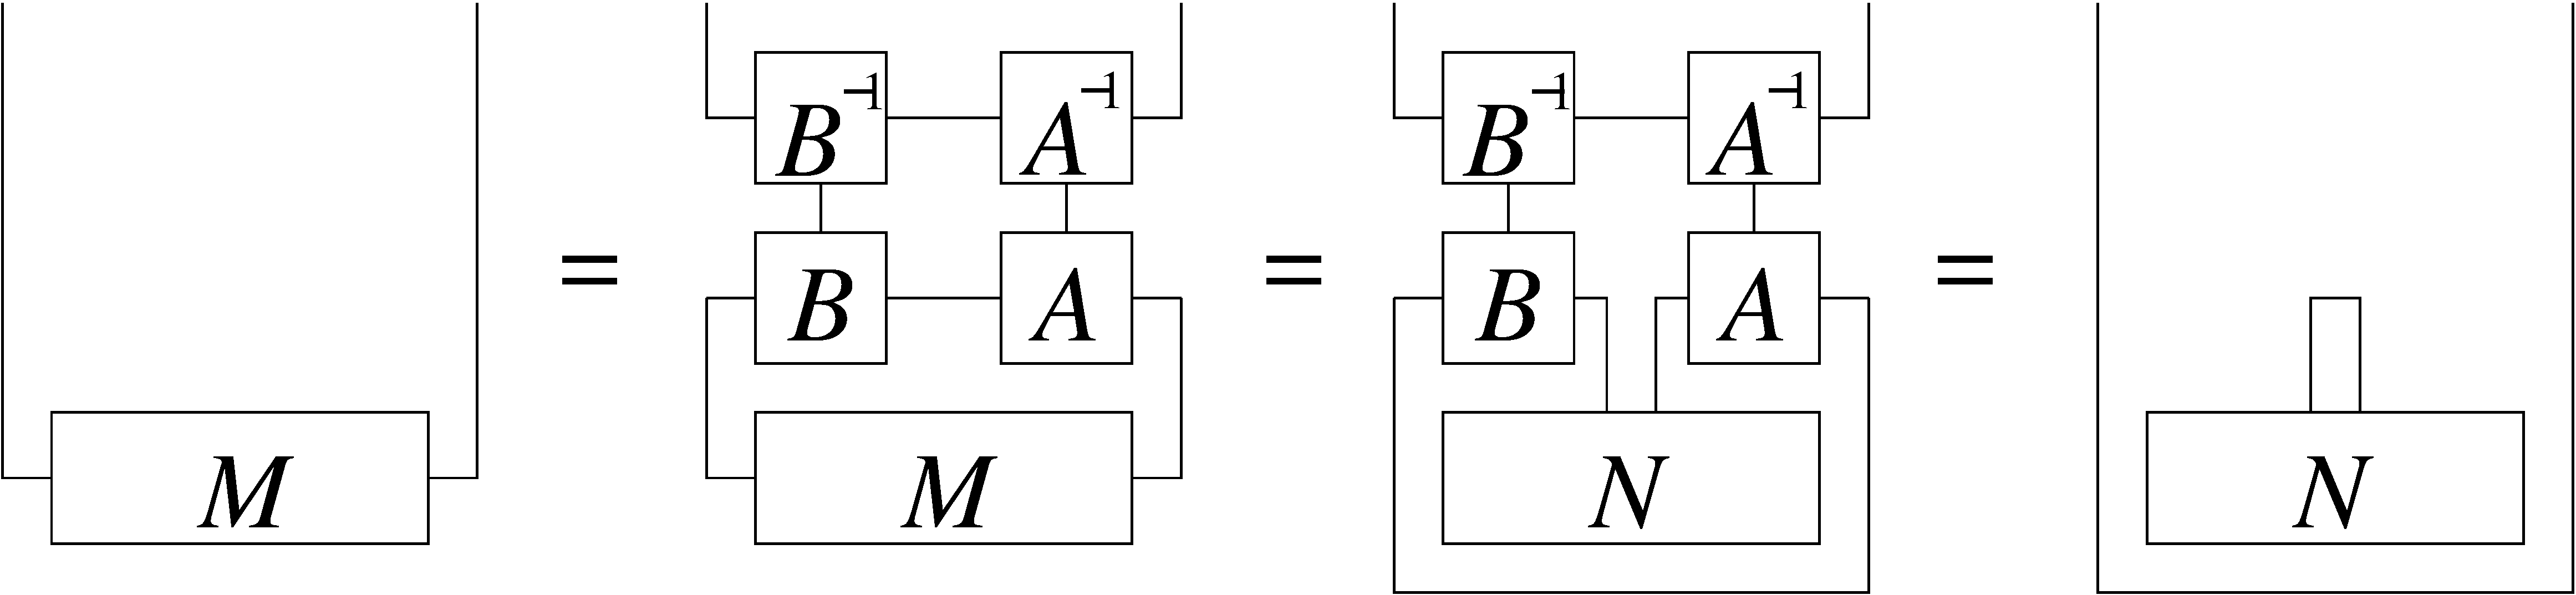
\includegraphics[height=5.5em]{diagrams/prove-inj-closure}\ ,
\]
shows that ${\rm lhs} \subseteq {\rm rhs}$.
Putting these inclusions together, we obtain {\rm lhs} = {\rm rhs}.
\end{proof}
\begin{theorem}[Parent Hamiltonian]
\label{thm:parent}
\end{theorem}
\begin{proof}
Take $B^\alpha = A^{i+1} \dots A^{L-1}$, with the index $\alpha=(i+1,\dots,L-1)$,
\[
  \mathcal{S}_{L-1} \otimes \mathbb{C}^d = \left\{\sum_{i_1,\alpha,i_L} \trace(A^{i_1} B^\alpha M^{i_{L}}) \ket{i_1,\alpha,i_{L}} \middle\vert M \in \mathbb{C}^d\otimes \mathbf{L}(\mathbb{C}^{D \times D}) \right\}
\]
and similarly for $\mathbb{C}^d \otimes \mathcal{S}_{L-1}$.
Then, applying the intersection property, $\mathcal{S}_L = \left(\mathcal{S}_{L-1} \otimes \mathbb{C}^d\right) \cap \left(\mathbb{C}^d \otimes \mathcal{S}_{L-1}\right)$.
By repeatedly  we span the whole space $\mathcal{S}_L$.
\[
  \mathcal{S}_L = 
  \left(\mathcal{S}_2 \otimes (\mathbb{C}^d)^{\otimes(L-2)}\right) \cap  \dots \cap \left((\mathbb{C}^d)^{\otimes(L-2)} \otimes \mathcal{S}_2 \right) = 
  \bigcap_{k=1}^{L-1} \, (\mathbb{C}^d)^{\otimes(k-1)} \otimes \mathcal{S}_2 \otimes (\mathbb{C}^d)^{\otimes(L-k-1)}
\]
Since $\mathcal{S}_2$ corresponds to the ground space of every $h_{i,i+1}$, $\mathcal{S}_L$ corresponds to the ground space of $H^\prime = \sum_{i=1}^{N-1} h_{i,i+1}$ (notice the open boundary conditions).
We now use. 
Now consider the ground spaces of the two operators $H_{\rm left} = h_{1,2} + \frac{1}{2} h_{2,3} + \dots  \frac{1}{2} h_{L-1,L}$
and $H_{\rm right} = \frac{1}{2} h_{2,3} + \dots  \frac{1}{2} h_{L-1,L} + h_{L,1}$.
The ground space of each of these operators is the lhs of Theorem~\ref{thm:closure}, from which we conclude that the ground space of $H_{\rm left} + H_{\rm right} = H$ is $\spanset\{\ket{\Psi}\}$.
\end{proof}
\end{section}
\end{document}
%%%%%%%%%%% Here Ends Document %%%%%%%%%%
